
%-----Appendix-------%
\appendix               	% at this point the appendix starts
\chapter{Organisation} 
\section{Project description} \label{PrjDescription} 
%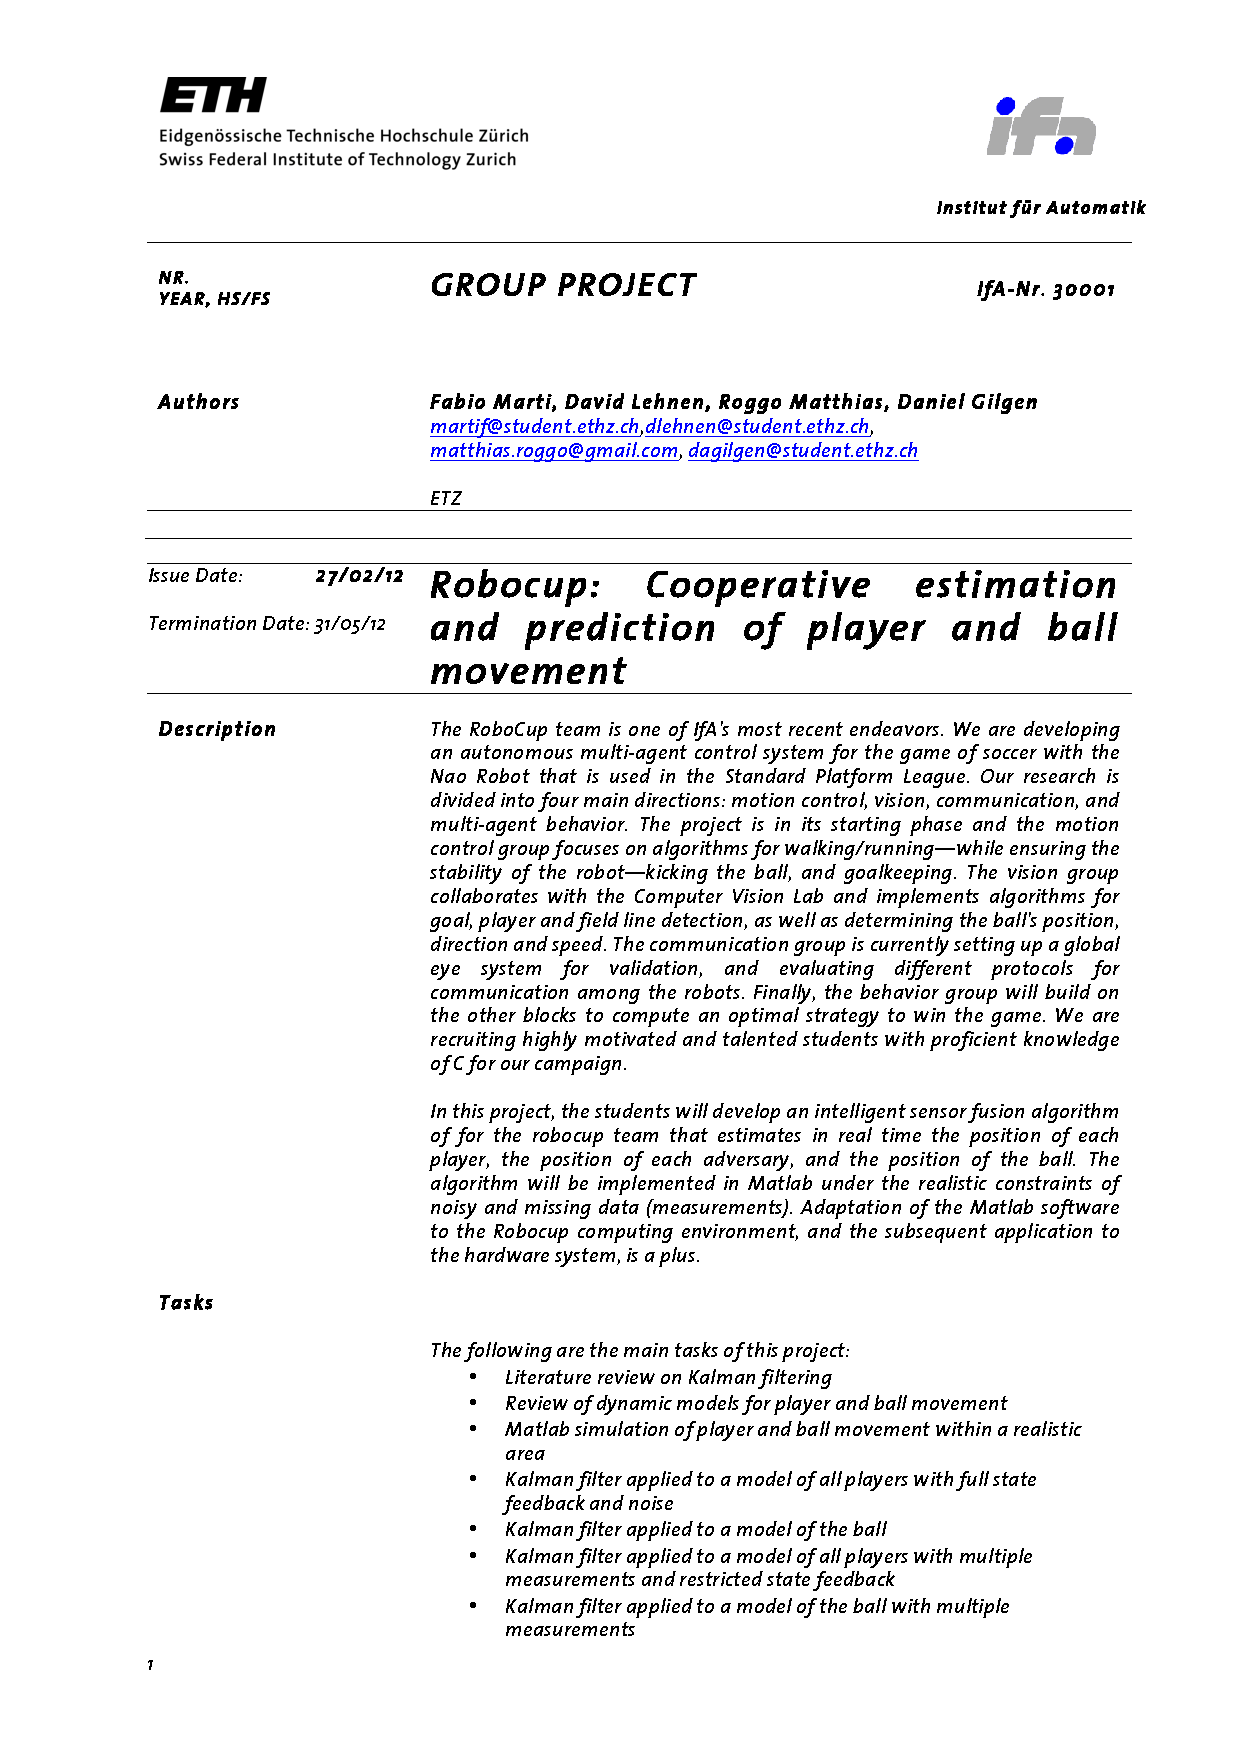
\includepdf[pages=-]{./appendix/Group_Project.pdf}

% -  -  -  -  -  -  -  -  -  -  -  -  -  -  -  -  -  -  -  -  -  -  -  -  -  -  -  -  -  -  -  -  -  -  -  -  -  -  -  -  -  -  -  -  -  -  -  -  -  -  -  -  - %
\section{MATLAB-Code Style Guidelines for our project}
In the MATLAB-Script \texttt{RoboCupSim.m} and in the associated functions we tried to use following naming convention:
\begin{itemize}
	\item \textbf{Variables}
		\begin{itemize}
			\item in general: \emph{mixed case starting with lower case}\\
				e.g. \texttt{goalHeight, dt}
			\item representing a number of objects: \emph{prefix n}\\
				e.g. \texttt{nSteps}
			\item iterator variables: \emph{prefix i,j,k}\\
				e.g. \texttt{iStep}
			\item boolean variables: \emph{prefix is}\\
				e.g. \texttt{isValid}
		\end{itemize}
	
	\item \textbf{Constants}: \emph{all uppercase using underscore to separate words}\\
		e.g. \texttt{MAX\_ITERATIONS}
	
	\item \textbf{Structures}: \emph{begin with a capital letter}\\
		e.g. \texttt{Field.width, Noise.Process.pos}
	
	\item \textbf{Functions}: \emph{lower case with underscore to separate words}\\
		e.g. \texttt{plot\_objects, ball\_step}
\end{itemize}


\chapter{Examples} 
\section{Kalman Filtering of Linear System} \label{ExampleKF} 
%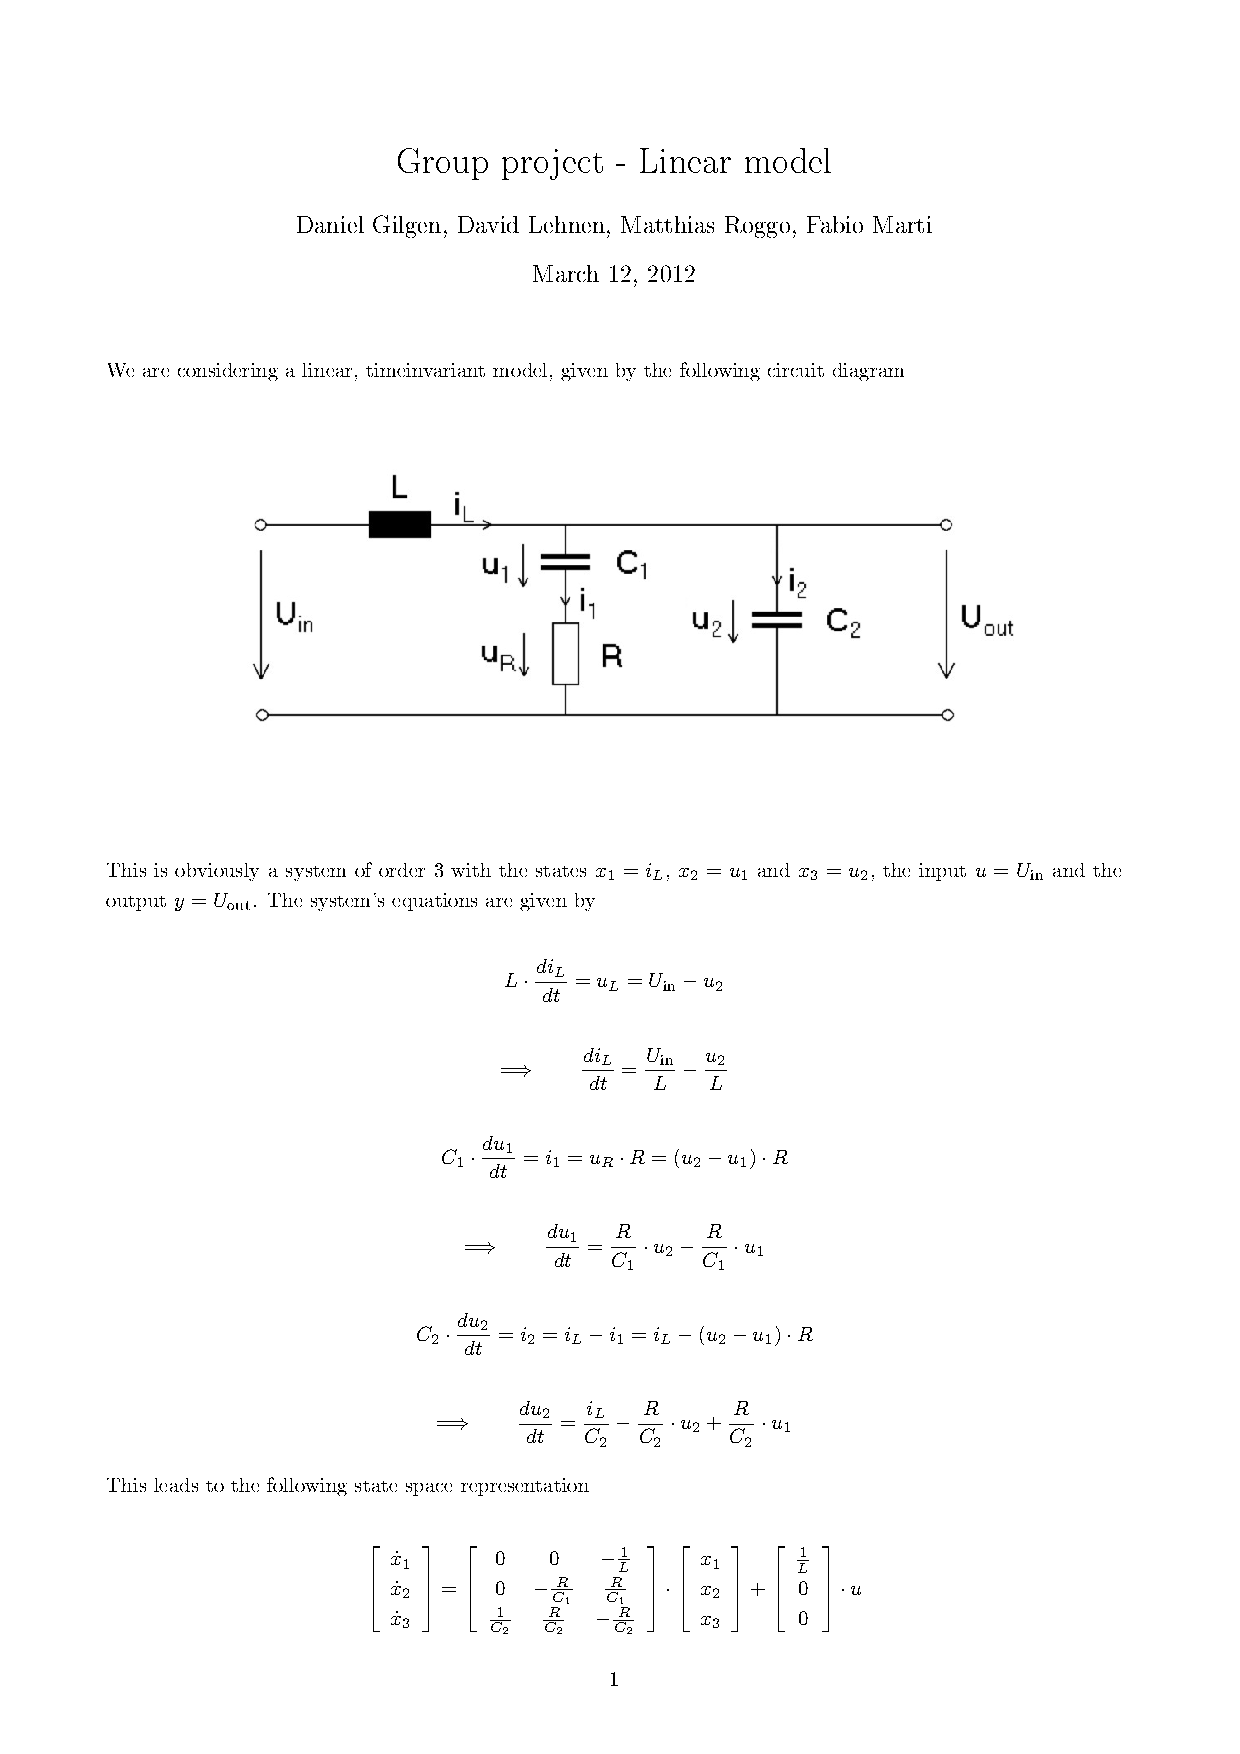
\includepdf[pages=-]{./appendix/linear_model.pdf}

\section{Kalman Filtering of Nonlinear System} \label{ExampleEKF}
%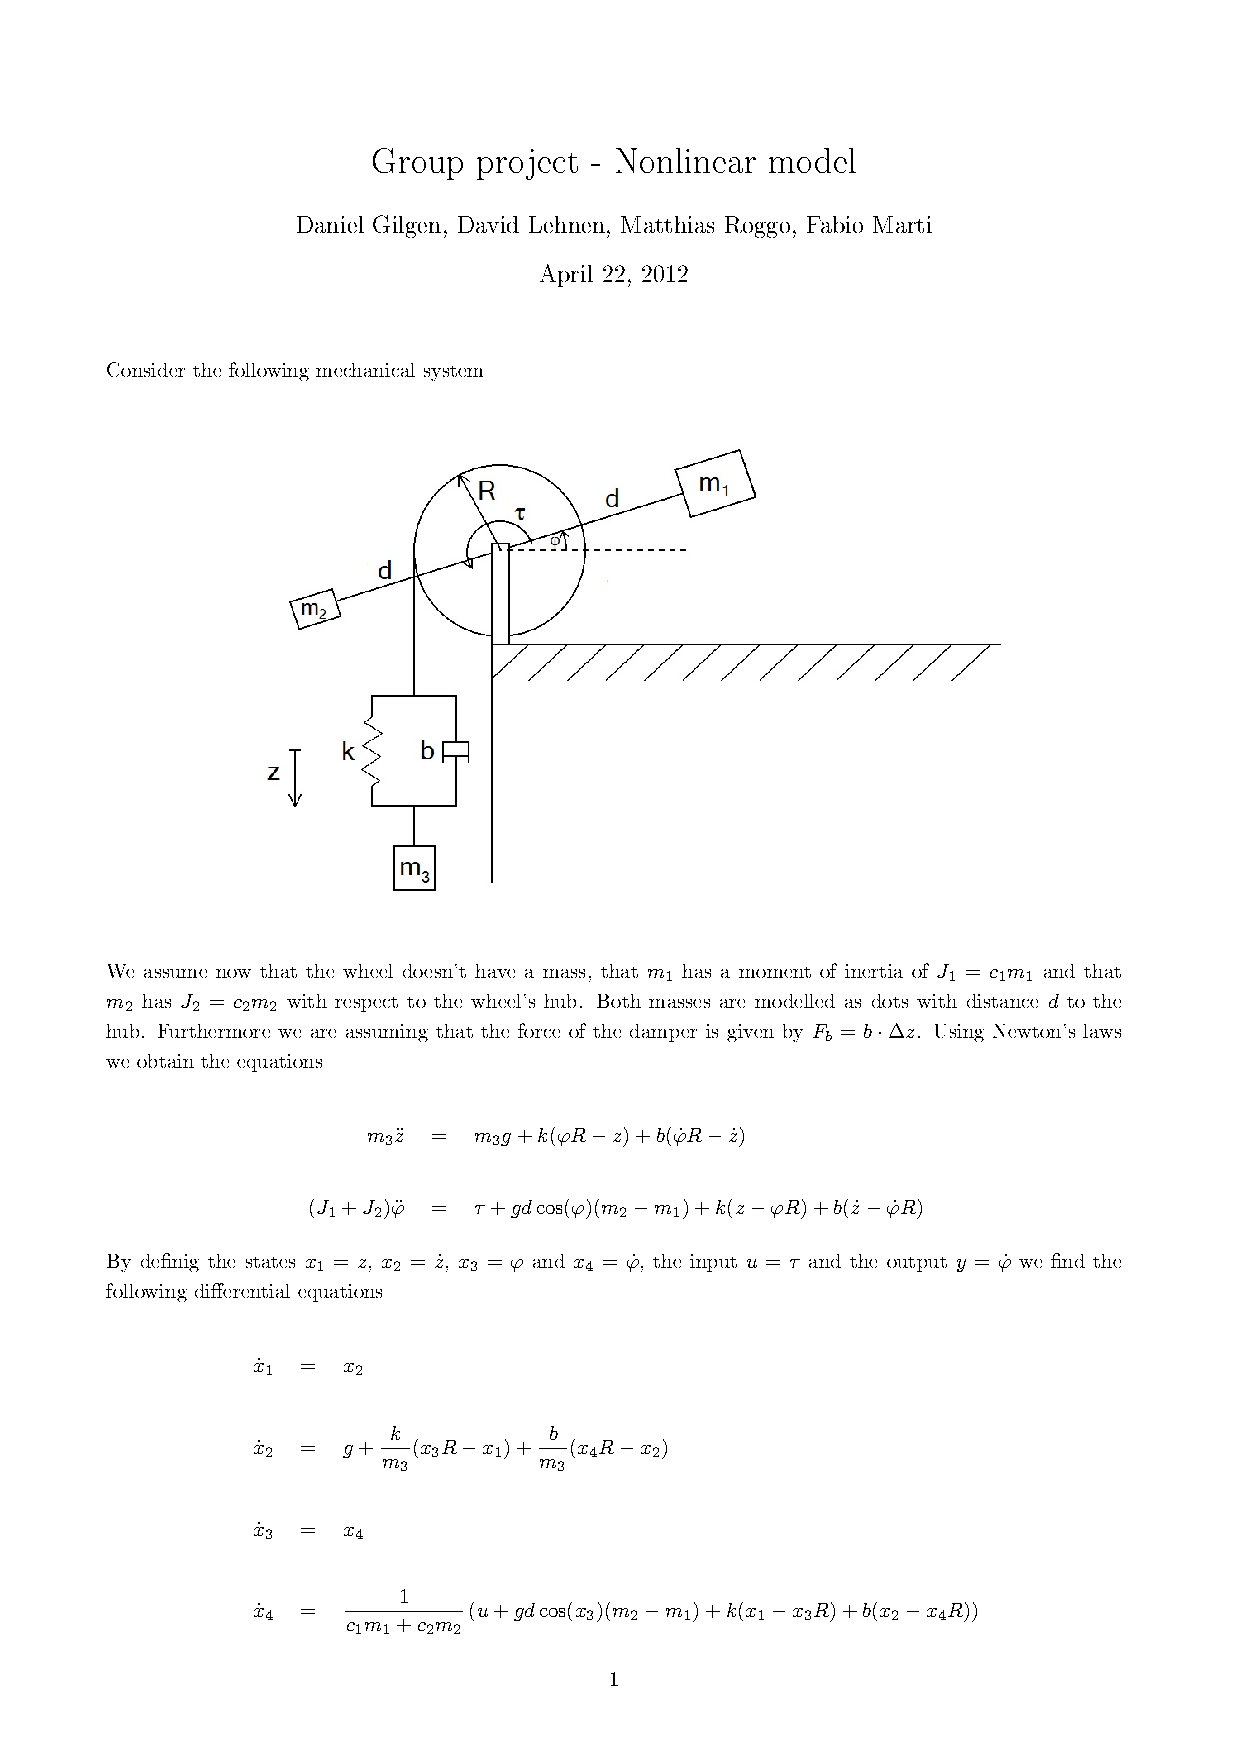
\includepdf[pages=-]{./appendix/nonlinear_model.pdf}